\section{Appendix}

In this appendix we provide implementation details and additional results. 
We optimize VAEs with Adam~\cite{kingma2014adam} with default parameters and learning rate $10^{-4}$. The $210 \times 160$ images are grayscaled and downsampled to $128 \times 128$. 
VAE-IW(1) experiments were performed with 4GB of RAM on one core of a Xeon Gold 6126 CPU, and a Tesla V100 GPU.
In \cref{tab:constant} we summarize the default hyperparameters of our main experiments, and in
\crefrange{tab:residualblock}{tab:decoder15} we detail the architectures of the VAEs. We used Bernoulli decoders, i.e. the reconstruction loss is the binary cross-entropy. 
Then, in \crefrange{tab:atari-model-comp}{tab:higher_time_budget_bprost} we report the results of our ablation studies on a subset of 47 games. While the main VAE-IW results (also reported in \cref{tab:atari-lookahead-0.5}) are averages of 10 runs, all other results in this appendix are averages of 5 runs. 
In \cref{tab:atari-piiw-rainbow} we compare our main results from \cref{tab:atari-lookahead-0.5} with $\pi$-IW \cite{RLIW} and Rainbow \cite{rainbow}, which is a DQN-based deep reinforcement learning algorithm. These comparisons are useful to get a sense of how VAE-IW stands against existing approaches for Atari, but should be taken with a grain of salt as these methods (especially Rainbow) differ significantly from VAE-IW.
Finally, Figures~\ref{fig:mean_expanded_nodes} and~\ref{fig:mean_depth_nodes} show additional statistics on the width-based search in terms of number of expanded nodes and their depth.

\vspace{5pt}
\begin{table}[ht]
    \centering
    \begin{tabular}{l l}
        \toprule
        \textbf{Parameter} & \textbf{Value} \\
        \midrule
        Batch size & 64\\
        Learning rate & $10^{-4}$\\
        Latent space size & $15 \times 15 \times 20 = 4500$ \\
        $\tau$ & 0.5\\
        $\beta$ & $10^{-4}$\\
        $\mu$ & $0.5$\\
        $\alpha$ & 50000\\
        $\gamma$ & 0.99 \\
        $\lambda$ & 0.9 \\
        Frame skip & 15\\
        Planning budget & 0.5s\\
        \bottomrule
    \end{tabular}
    \caption{Default hyperparameters for VAE-IW experiments.}
    \label{tab:constant}
\end{table}
\begin{table}[ht]
    \centering % \small
    \begin{tabular}{l}
        \toprule
        \textbf{Residual block}\\
        \midrule
        BatchNorm\\
        LeakyReLU(0.01)\\
        Conv $3 \times 3$, 64 channels, padding=1\\
        Dropout(0.2)\\
        BatchNorm\\
        LeakyReLU(0.01)\\
        Conv $3 \times 3$, 64 channels, padding=1\\
        Dropout(0.2)\\
        Add to block input \\
        LeakyReLU(0.01)\\
        \bottomrule
    \end{tabular}
    \caption{Architecture of a residual block.}
    \label{tab:residualblock}
\end{table}
\begin{table}[ht]
    \centering %\small
    \begin{tabular}{l}
        \toprule
        \textbf{Encoder $4 \times 4$}\\
        \midrule
        Conv $3 \times 3$, 64 channels, stride=2\\
        Residual block\\
        Conv $3 \times 3$, 64 channels, stride=2\\
        Residual block\\
        Conv $3 \times 3$, 64 channels, stride=2\\
        Residual block\\
        Conv $3 \times 3$, 64 channels, stride=2\\
        Residual block\\
        Conv $3 \times 3$, $200$ channels, stride=2, padding=1\\
        \bottomrule
    \end{tabular}
    \caption{Encoder with output of spatial size $4\times 4$.}
    \label{tab:encoder4}
\end{table}
\begin{table}[ht]
    \centering % \small
    \begin{tabular}{l}
        \toprule
        \textbf{Decoder $4 \times 4$}\\
        \midrule
        ConvT $3 \times 3$, 64 channels, stride=2\\
        Residual block\\
        ConvT $3 \times 3$, 64 channels, stride=2\\
        Residual block\\
        ConvT $3 \times 3$, 64 channels, stride=2\\
        Residual block\\
        ConvT $3 \times 3$, 64 channels, stride=2\\
        Residual block\\
        ConvT $3 \times 3$, 1 channel, stride=2\\
        Crop $128 \times 128$ \\
        Sigmoid\\
        \bottomrule
    \end{tabular}
    \caption{Decoder with input of spatial size $4\times 4$. ConvT denotes transposed convolutional layers.}
    \label{tab:decoder4}
\end{table}
\begin{table}[ht]
    \centering % \small
    \begin{tabular}{l}
        \toprule
        \textbf{Encoder $15 \times 15$}\\
        \midrule
        Conv $4 \times 4$, 64 channels, stride=2\\
        Residual block\\
        Conv $4 \times 4$, 64 channels, stride=2\\
        Residual block\\
        Conv $3 \times 3$, $20$ channels, stride=2, padding=1\\
        \bottomrule
    \end{tabular}
    \caption{Encoder with output of spatial size $15\times 15$.}
    \label{tab:encoder15}
\end{table}
\begin{table}[ht]
    \centering % \small
    \begin{tabular}{l}
        \toprule
        \textbf{Decoder $15 \times 15$}\\
        \midrule
        ConvT $3 \times 3$, 64 channels, stride=2\\
        Residual block\\
        ConvT $4 \times 4$, 64 channels, stride=2\\
        Residual block\\
        ConvT $4 \times 4$, 1 channel, stride=2\\
        Crop $128 \times 128$ \\
        Sigmoid\\
        \bottomrule
    \end{tabular}
    \caption{Decoder with input of spatial size $15\times 15$. ConvT denotes transposed convolutional layers.}
    \label{tab:decoder15}
\end{table}


\begin{table}[ht]
\begin{center}
\begin{small}
%\begin{sc}
\begin{tabular}{lrrrrrrrl}

\toprule
Algorithm& RA VAE-IW & RA VAE-IW \\
    $\beta$ & $10^{-4}$ & $10^{-4}$\\
Planning horizon&  0.5s & 0.5s \\
Features &   VAE $15 \times 15 \times 20$ &  VAE $4 \times 4 \times 200$ \\
\midrule
Alien           & \textbf{7,744.0}     & 7,592.0              \\
Amidar          & 1,380.3              & \textbf{1,526.6}     \\
Assault         & 1,291.9              & \textbf{1,308.6}     \\
Asterix         & \textbf{999,500.0}   & \textbf{999,500.0}   \\
Asteroids       & \textbf{12,647.0}    & 8,852.0              \\
Atlantis        & \textbf{1,977,520.0*} & 1,912,700.0*          \\
Battle zone     & 115,400.0            & \textbf{228,000.0}   \\
Beam rider      & \textbf{3,792.0}     & 3,450.0              \\
Berzerk         & \textbf{863.0}       & 752.0                \\
Bowling         & \textbf{54.4}        & 47.6                 \\
Breakout        & \textbf{45.7}        & 28.4                 \\
Centipede       & \textbf{428,451.5*}   & 253,823.6*            \\
Crazy climber   & 901,930.0*            & \textbf{930,420.0*}   \\
Demon attack    & 285,867.5*            & \textbf{292,099.0*}   \\
Double dunk     & \textbf{8.6}         & 6.0                  \\
Elevator action & 40,000.0*             & \textbf{109,680.0*}   \\
Fishing derby   & \textbf{-20.0}       & -31.2                \\
Freeway         & \textbf{5.3}         & 2.0                  \\
Frostbite       & \textbf{259.0}       & 244.0                \\
Gopher          & 8,484.0              & \textbf{8,504.0}     \\
Gravitar        & \textbf{1,940.0}     & 1,560.0              \\
Ice hockey      & \textbf{37.2}        & \textbf{37.2}        \\
James bond 007  & 3,035.0              & \textbf{11,000.0}    \\
Krull           & \textbf{3,433.9}     & 3,219.0              \\
Kung-fu master  & \textbf{4,550.0}     & 3,600.0              \\
Ms. Pac-man     & \textbf{17,929.8}    & 15,066.8             \\
Name this game  & \textbf{17,374.0}    & 13,670.0             \\
Phoenix         & 5,919.0              & \textbf{9,210.0}     \\
Pitfall!        & \textbf{-5.6}        & -9.6                 \\
Pong            & \textbf{4.2}         & 3.6                  \\
Private eye     & 80.0                 & \textbf{115.4}       \\
Q*bert          & 3,392.5              & \textbf{4,935.0}     \\
River raid      & 6,701.0              & \textbf{6,790.0}     \\
Road Runner     & \textbf{2,980.0}     & 2,320.0              \\
Robotank        & 25.6                 & \textbf{45.2}        \\
Seaquest        & 842.0                & \textbf{1,084.0}     \\
Skiing          & \textbf{-10,046.9}   & -11,906.4            \\
Space invaders  & 2,574.0              & \textbf{2,753.0}     \\
Stargunner      & 1,030.0              & \textbf{1,200.0}     \\
Tennis          & \textbf{4.1}         & -6.6                 \\
Time pilot      & \textbf{32,840.0}    & 23,460.0             \\
Tutankham       & \textbf{177.0}       & 158.4                \\
Up'n down       & \textbf{762,453.0*}   & 627,706.0*            \\
Video pinball   & \textbf{373,914.3}   & 248,101.2            \\
Wizard of wor   & \textbf{199,900.0*}   & 111,580.0            \\
Yars' revenge   & 96,053.3             & \textbf{97,004.6}    \\
Zaxxon          & 15,560.0             & \textbf{17,360.0}    \\
\midrule

\# best & 29 & 20  \\

\bottomrule

\end{tabular}
%\end{sc}
\end{small}
\end{center}
\caption{Score comparison of VAE-IW with latent space size $15\times15\times20$ and $4\times4\times 200$. Scores in bold indicate the best method, and scores with a star indicate that the algorithm reached the limit on executed actions at least once. Ties are counted as won for both methods.} 
\label{tab:atari-model-comp}
\end{table}
\begin{table}
% \begin{center}
\centering

\resizebox{\columnwidth}{!}{%
\begin{tabular}{lrrrrrrrl}

\toprule
Algorithm & RA VAE-IW & RA VAE-IW & RA VAE-IW \\
Model type & Continuous & Continuous & Discrete \\
Quantization & 6 bits & 4 bits & --- \\
% Planning budget& & 0.5s & 0.5s &  0.5s  \\

\midrule
Alien          & 6,988.0              & 7,532.0              & \textbf{7,744.0}     \\
Amidar         & 784.0                & 612.2                & \textbf{1,380.3}     \\
Assault        & 1,286.0              & \textbf{1,357.4}     & 1,291.9              \\
Asterix        & \textbf{999,500.0*}   & \textbf{999,500.0*}   & \textbf{999,500.0*}   \\
Asteroids      & 2,886.0              & 2,670.0              & \textbf{12,647.0}    \\
Atlantis       & \textbf{1,999,040.0*} & 1,997,760.0 *         & 1,977,520.0*          \\
BattleZone     & 90,800.0             & 83,400.0             & \textbf{115,400.0}   \\
BeamRider      & \textbf{4,380.0}     & 3,810.0              & 3,792.0              \\
Berzerk        & \textbf{1,032.0}     & \textbf{1,032.0}     & 863.0                \\
Bowling        & 48.4                 & 43.4                 & \textbf{54.4}        \\
Breakout       & 73.2                 & \textbf{158.4}       & 45.7                 \\
Centipede      & 1,191,414.0*          & \textbf{1,214,556.4*} & 428,451.5*            \\
CrazyClimber   & 225,980.0*            & 264,160.0*            & \textbf{901,930.0*}   \\
DemonAttack    & 291,138.0*            & \textbf{299,555.0*}   & 285,867.5*            \\
DoubleDunk     & 3.4                  & 0.2                  & \textbf{8.6}         \\
ElevatorAction & 35,580.0             & 38,000.0             & \textbf{40,000.0}    \\
FishingDerby   & -26.2                & -25.6                & \textbf{-20.0}       \\
Freeway        & 7.8                  & \textbf{8.2}         & 5.3                  \\
Frostbite      & \textbf{282.0}       & 238.0                & 259.0                \\
Gopher         & 6,772.0              & 7,580.0              & \textbf{8,484.0}     \\
Gravitar       & 1,840.0              & \textbf{3,380.0}     & 1,940.0              \\
IceHockey      & 29.0                 & 34.8                 & \textbf{37.2}        \\
Jamesbond      & 780.0                & 1,500.0              & \textbf{3,035.0}     \\
Krull          & 3,175.8              & \textbf{3,625.2}     & 3,433.9              \\
KungFuMaster   & \textbf{6,740.0}     & \textbf{6,740.0}     & 4,550.0              \\
MsPacman       & \textbf{24,555.0}    & 17,630.8             & 17,929.8             \\
NameThisGame   & \textbf{17,594.0}    & 16,046.0             & 17,374.0             \\
Phoenix        & 5,532.0              & 5,902.0              & \textbf{5,919.0}     \\
Pitfall        & -9.6                 & -47.8                & \textbf{-5.6}        \\
Pong           & 1.8                  & \textbf{4.6}         & 4.2                  \\
PrivateEye     & -102.6               & -107.8               & \textbf{80.0}        \\
Qbert          & 2,795.0              & \textbf{5,575.0}     & 3,392.5              \\
Riverraid      & \textbf{7,838.0}     & 7,382.0              & 6,701.0              \\
RoadRunner     & 2,600.0              & \textbf{6,900.0}     & 2,980.0              \\
Robotank       & \textbf{34.8}        & 23.6                 & 25.6                 \\
Seaquest       & \textbf{3,852.0}     & 2,016.0              & 842.0                \\
Skiing         & -28,186.0            & -29,598.6            & \textbf{-10,046.9}   \\
SpaceInvaders  & 2,058.0              & 1,862.0              & \textbf{2,574.0}     \\
StarGunner     & 1,180.0              & \textbf{1,400.0}     & 1,030.0              \\
Tennis         & -1.8                 & 0.4                  & \textbf{4.1}         \\
TimePilot      & 21,300.0             & 23,500.0             & \textbf{32,840.0}    \\
Tutankham      & 162.4                & 157.2                & \textbf{177.0}       \\
UpNDown        & 850,624.0*            & \textbf{862,708.0*}   & 762,453.0*            \\
VideoPinball   & 370,304.6            & \textbf{477,225.2}   & 373,914.3            \\
WizardOfWor    & 109,140.0            & 151,060.0            & \textbf{199,900.0*}   \\
YarsRevenge    & 117,236.2            & \textbf{137,892.4}   & 96,053.3             \\
Zaxxon         & 15,260.0             & \textbf{15,860.0}    & 15,560.0             \\
\midrule

\# best in game & 10 & 18 & 23 \\
\bottomrule
\end{tabular}%
}
% \end{center}
\caption{Score comparison of RA VAE-IW with discrete (default model with latent space of size $15 \times 15 \times 20 = 4500$) and continuous random variables. In the continuous case, the latent space has size $15 \times 15 \times 5$, and then each random variable is quantized in $2^4$ or $2^6$ bins with equal probability under the prior. This leads to 4 or 6 bits per random variable, and hence 4,500 and 6,750 binary features, respectively. All other parameters are the default ones from the main text.
} 
\label{tab:continuous}
\end{table}


\begin{table}[ht]
\begin{center}
\begin{small}
%\begin{sc}
\begin{tabular}{lrrrl}

\toprule
Algorithm  & RA VAE-IW & RA VAE-IW \\
$\beta$ & $10^{-3}$ & $10^{-4}$\\
Planning horizon & 0.5s & 0.5s  \\
Features &  VAE $15 \times 15 \times 20$ &  VAE $15 \times 15 \times 20$ \\
\midrule

Alien           & 4,902.0              & \textbf{7,744.0}     \\
Amidar          & 1,186.2              & \textbf{1,380.3}     \\
Assault         & \textbf{1,468.2}     & 1,291.9              \\
Asterix         & \textbf{999,500.0*}   & \textbf{999,500.0*}   \\
Asteroids       & 7,204.0              & \textbf{12,647.0}    \\
Atlantis        & \textbf{1,978,540.0*} & 1,977,520.0*          \\
Battle zone     & \textbf{406,600.0}   & 115,400.0            \\
Beam rider      & \textbf{4,377.6}     & 3,792.0              \\
Berzerk         & 774.0                & \textbf{863.0}       \\
Bowling         & 35.0                 & \textbf{54.4}        \\
Breakout        & \textbf{53.4}        & 45.7                 \\
Centipede       & 296,791.4*           & \textbf{428,451.5*}   \\
Crazy climber   & \textbf{976,580.0*}   & 901,930.0*            \\
Demon attack    & \textbf{301,886.0*}   & 285,867.5*            \\
Double dunk     & 7.4                  & \textbf{8.6}         \\
Elevator action & \textbf{68,920.0*}    & 40,000.0*             \\
Fishing derby   & \textbf{-15.6}       & -20.0                \\
Freeway         & 4.0                  & \textbf{5.3}         \\
Frostbite       & \textbf{262.0}       & 259.0                \\
Gopher          & 5,420.0              & \textbf{8,484.0}     \\
Gravitar        & \textbf{2,300.0}     & 1,940.0              \\
Ice hockey      & 34.0                 & \textbf{37.2}        \\
James bond 007  & 630.0                & \textbf{3,035.0}     \\
Krull           & \textbf{3,486.4}     & 3,433.9              \\
Kung-fu master  & \textbf{4,960.0}     & 4,550.0              \\
Ms. Pac-man     & 17,483.0             & \textbf{17,929.8}    \\
Name this game  & 15,120.0             & \textbf{17,374.0}    \\
Phoenix         & 5,524.0              & 5,919.0              \\
Pitfall!        & -6.8                 & \textbf{-5.6}        \\
Pong            & -2.2                 & \textbf{4.2}         \\
Private eye     & 40.0                 & \textbf{80.0}        \\
Q*bert          & \textbf{8,040.0}     & 3,392.5              \\
River raid      & 6,078.0              & \textbf{6,701.0}     \\
Road Runner     & 2,080.0              & \textbf{2,980.0}     \\
Robotank        & \textbf{44.6}        & 25.6                 \\
Seaquest        & 316.0                & \textbf{842.0}       \\
Skiing          & -11,027.6            & \textbf{-10,046.9}   \\
Space invaders  & \textbf{2,721.0}     & 2,574.0              \\
Stargunner      & \textbf{1,100.0}     & 1,030.0              \\
Tennis          & -16.6                & \textbf{4.1}         \\
Time pilot      & 30,920.0             & \textbf{32,840.0}    \\
Tutankham       & 165.8                & \textbf{177.0}       \\
Up'n down       & 682,080.0*            & \textbf{762,453.0*}   \\
Video pinball   & \textbf{445,085.8}   & 373,914.3            \\
Wizard of wor   & 184,260.0            & \textbf{199,900.0*}   \\
Yars' revenge   & 77,950.8             & \textbf{96,053.3}    \\
Zaxxon          & 10,520.0             & \textbf{15,560.0}    \\

\midrule

\# best &    19                   & 29                      \\

\bottomrule

\end{tabular}
%\end{sc}
\end{small}
\end{center}
\caption{Score comparison of RA VAE-IW with different values of $\beta$. Scores in bold indicate the best method, and scores with a star indicate that the algorithm reached the limit on executed actions at least once. Ties are counted as won for both methods.} 
\label{tab:atari-comparison}
\end{table}

\begin{table}[ht]
\begin{center}
\begin{small}
%\begin{sc}
\begin{tabular}{lrrrrrrrl}
\toprule
Algorithm& VAE-IW & RA VAE-IW \\
$\beta$ & $10^{-4}$ & $10^{-4}$\\
Planning horizon& 0.5s & 0.5s  \\
Features & VAE $15 \times 15 \times 20$ & VAE $15 \times 15 \times 20$\\


\midrule

Alien           & 5,576.0              & \textbf{7,744.0}     \\
Amidar          & 1,093.2              & \textbf{1,380.3}     \\
Assault         & 826.4                & \textbf{1,291.9}     \\
Asterix         & \textbf{999,500.0*}   & \textbf{999,500.0*}   \\
Asteroids       & 772.0                & \textbf{12,647.0}    \\
Atlantis        & 40,620.0             & \textbf{1,977,520.0*} \\
Battle zone     & 91,200.0             & \textbf{115,400.0}   \\
Beam rider      & 3,179.6              & \textbf{3,792.0}     \\
Berzerk         & 566.0                & \textbf{863.0}       \\
Bowling         & \textbf{64.6}        & 54.4                 \\
Breakout        & 13.0                 & \textbf{45.7}        \\
Centipede       & 22,020.2             & \textbf{428,451.5*}   \\
Crazy climber   & 661,460.0            & \textbf{901,930.0*}   \\
Demon attack    & 9,656.0              & \textbf{285,867.5*}   \\
Double dunk     & 7.2                  & \textbf{8.6}         \\
Elevator action & \textbf{76,160.0*}    & 40,000.0*             \\
Fishing derby   & -20.2                & \textbf{-20.0}       \\
Freeway         & \textbf{6.2}         & 5.3                  \\
Frostbite       & 248.0                & \textbf{259.0}       \\
Gopher          & 6,084.0              & \textbf{8,484.0}     \\
Gravitar        & \textbf{2,770.0}     & 1,940.0              \\
Ice hockey      & 36.0                 & \textbf{37.2}        \\
James bond 007  & 640.0                & \textbf{3,035.0}     \\
Krull           & \textbf{3,543.2}     & 3,433.9              \\
Kung-fu master  & \textbf{5,160.0}     & 4,550.0              \\
Ms. Pac-man     & \textbf{20,161.0}    & 17,929.8             \\
Name this game  & 13,332.0             & \textbf{17,374.0}    \\
Phoenix         & 5,328.0              & \textbf{5,919.0}     \\
Pitfall!        & \textbf{0.0}         & -5.6                 \\
Pong            & \textbf{9.2}         & 4.2                  \\
Private eye     & \textbf{139.0}       & 80.0                 \\
Q*bert          & 1,890.0              & \textbf{3,392.5}     \\
River raid      & 4,884.0              & \textbf{6,701.0}     \\
Road Runner     & \textbf{4,720.0}     & 2,980.0              \\
Robotank        & 21.4                 & \textbf{25.6}        \\
Seaquest        & 596.0                & \textbf{842.0}       \\
Skiing          & \textbf{-9,664.8}    & -10,046.9            \\
Space invaders  & 1,962.0              & \textbf{2,574.0}     \\
Stargunner      & \textbf{1,120.0}     & 1,030.0              \\
Tennis          & \textbf{5.2}         & 4.1                  \\
Time pilot      & 24,840.0             & \textbf{32,840.0}    \\
Tutankham       & 167.4                & \textbf{177.0}       \\
Up'n down       & 35,964.0             & \textbf{762,453.0*}   \\
Video pinball   & \textbf{462,619.4}   & 373,914.3            \\
Wizard of wor   & 89,380.0             & \textbf{199,900.0*}   \\
Yars' revenge   & 85,800.6             & \textbf{96,053.3}    \\
Zaxxon          & 7,320.0              & \textbf{15,560.0}    \\

\midrule

\# best & 16 &  32 \\

\bottomrule

\end{tabular}
%\end{sc}
\end{small}
\end{center}
\caption{Score  comparison  of  VAE-IW  with  and  without risk aversion. Scores in bold indicate the best method, and scores with a star indicate that the algorithm reached the limit on executed actions at least once. Ties are counted as won for both methods. } 
\label{tab:atari-ra_no-ra}
\end{table}



\begin{table}[ht]
\begin{center}
\begin{small}
%\begin{sc}
\begin{tabular}{lrrl}
\toprule
Algorithm& Rollout IW & VAE-IW \\
$\beta$ &  & $10^{-4}$\\
Planning horizon& 0.5s & 0.5s  \\
Features & B-PROST & VAE $15 \times 15 \times 20$\\

\midrule

Alien           & 4,238.0           & \textbf{5,576.0}   \\
Amidar          & 659.8             & \textbf{1,093.2}   \\
Assault         & 285.0             & \textbf{826.4}     \\
Asterix         & 45,780.0          & \textbf{999,500.0} \\
Asteroids       & \textbf{4,344.0}  & 772.0              \\
Atlantis        & \textbf{64,200.0} & 40,620.0           \\
Battle zone     & 39,600.0          & \textbf{91,200.0}  \\
Beam rider      & 2,188.0           & \textbf{3,179.6}   \\
Berzerk         & \textbf{644.0}    & 566.0              \\
Bowling         & 47.6              & \textbf{64.6}      \\
Breakout        & \textbf{82.4}     & 13.0               \\
Centipede       & \textbf{36,980.2} & 22,020.2           \\
Crazy climber   & 39,220.0          & \textbf{661,460.0*} \\
Demon attack    & 2,780.0           & \textbf{9,656.0}   \\
Double dunk     & 3.6               & \textbf{7.2}       \\
Elevator action & 0.0               & \textbf{76,160.0*}  \\
Fishing derby   & -68.0             & \textbf{-20.2}     \\
Freeway         & 2.8               & \textbf{6.2}       \\
Frostbite       & 220.0             & \textbf{248.0}     \\
Gopher          & \textbf{7,216.0}  & 6,084.0            \\
Gravitar        & 1,630.0           & \textbf{2,770.0}   \\
Ice hockey      & -6.0              & \textbf{36.0}      \\
James bond 007  & 450.0             & \textbf{640.0}     \\
Krull           & 1,892.8           & \textbf{3,543.2}   \\
Kung-fu master  & 2,080.0           & \textbf{5,160.0}   \\
Ms. Pac-man     & 9,178.4           & \textbf{20,161.0}  \\
Name this game  & 6,226.0           & \textbf{13,332.0}  \\
Phoenix         & \textbf{5,750.0}  & 5,328.0            \\
Pitfall!        & -81.4             & \textbf{0.0}       \\
Pong            & -7.4              & \textbf{9.2}       \\
Private eye     & -322.0            & \textbf{139.0}     \\
Q*bert          & \textbf{3,375.0}  & 1,890.0            \\
River raid      & \textbf{6,088.0}  & 4,884.0            \\
Road Runner     & 2,360.0           & \textbf{4,720.0}   \\
Robotank        & \textbf{31.0}     & 21.4               \\
Seaquest        & \textbf{980.0}    & 596.0              \\
Skiing          & -15,738.8         & \textbf{-9,664.8}  \\
Space invaders  & \textbf{2,628.0}  & 1,962.0            \\
Stargunner      & \textbf{13,360.0} & 1,120.0            \\
Tennis          & -18.6             & \textbf{5.2}       \\
Time pilot      & 7,640.0           & \textbf{24,840.0}  \\
Tutankham       & 128.4             & \textbf{167.4}     \\
Up'n down       & \textbf{36,236.0} & 35,964.0           \\
Video pinball   & 203,765.4         & \textbf{462,619.4} \\
Wizard of wor   & 37,220.0          & \textbf{89,380.0}  \\
Yars' revenge   & 5,225.4           & \textbf{85,800.6}  \\
Zaxxon          & \textbf{9,280.0}  & 7,320.0           \\

\midrule

\# best & 15 &  32 \\

\bottomrule

\end{tabular}
%\end{sc}
\end{small}
\end{center}
\caption{Score comparison between RolloutIW B-PROST and VAE-IW, both without risk aversion. Scores in bold indicate the best method, and scores with a star indicate that the algorithm reached the limit on executed actions at least once. Ties are counted as won for both methods.} 
\label{tab:atari-no-ra}
\end{table}

\begin{table}[ht]
    \centering
\begin{center}
\begin{small}
\begin{tabular}{lrr}
\toprule
Algorithm & VAE-IW & VAE-IW \\
$\beta$ & $10^{-4}$ & $10^{-4}$\\
Planning horizon & 0.5s & 32s \\
Features &  VAE $15 \times 15 \times 20$ &  VAE $15 \times 15 \times 20$ \\
\midrule


Alien          & 5,576.0            & \textbf{8,536.0}   \\
Amidar         & 1,093.2            & \textbf{1,955.8}   \\
Assault        & 826.4              & \textbf{1,338.4}   \\
Asterix        & \textbf{999,500.0} & \textbf{999,500.0}         \\
Asteroids      & 772.0              & \textbf{1,158.0}   \\
Atlantis       & 40,620.0           & \textbf{49,500.0}  \\
BattleZone     & 91,200.0           & \textbf{234,200.0} \\
BeamRider      & 3,179.6            & \textbf{5,580.0}   \\
Berzerk        & \textbf{566.0}     & 554.0              \\
Bowling        & \textbf{64.6}      & 46.8               \\
Breakout       & 13.0               & \textbf{72.4}      \\
Centipede      & 22,020.2           & \textbf{166,244.8} \\
CrazyClimber   & 661,460.0          & \textbf{731,867.2}  \\
DemonAttack    & \textbf{9,656.0}   & 5,397.0            \\
DoubleDunk     & \textbf{7.2}       & 5.2                \\
ElevatorAction & 76,160.0           & \textbf{88,100.0}     \\
FishingDerby   & -20.2              & \textbf{20.6}      \\
Freeway        & 6.2                & \textbf{29.4}      \\
Frostbite      & 248.0              & \textbf{280.0}     \\
Gopher         & 6,084.0            & \textbf{17,604.0}  \\
Gravitar       & \textbf{2,770.0}   & 2,640.0            \\
IceHockey      & 36.0               & \textbf{44.2}      \\
Jamesbond      & 640.0              & \textbf{650.0}     \\
Krull          & 3,543.2            & \textbf{6,664.0}   \\
KungFuMaster   & 5,160.0            & \textbf{20,960.0}  \\
MsPacman       & 20,161.0           & \textbf{25,759.0}  \\
NameThisGame   & 13,332.0           & \textbf{15,276.0}  \\
Phoenix        & 5,328.0            & \textbf{5,960.0}   \\
Pitfall        & \textbf{0.0}       & -0.4               \\
Pong           & 9.2                & \textbf{12.0}      \\
PrivateEye     & 139.0              & \textbf{157.8}     \\
Qbert          & 1,890.0            & \textbf{4,760.0}   \\
Riverraid      & 4,884.0            & \textbf{5,372.0}   \\
RoadRunner     & 4,720.0            & \textbf{8,540.0}   \\
Robotank       & 21.4               & \textbf{24.2}      \\
Seaquest       & \textbf{596.0}     & 324.0              \\
Skiing         & \textbf{-9,664.8}  & -9,705.0           \\
SpaceInvaders  & 1,962.0            & \textbf{2,972.0}   \\
StarGunner     & {1,120.0}          & \textbf{1,180.0}   \\
Tennis         & {5.2}              & \textbf{12.6}      \\
TimePilot      & \textbf{24,840.0}  & 24,220.0           \\
Tutankham      & 167.4              & \textbf{197.2}     \\
UpNDown        & 35,964.0           & \textbf{91,592.0}  \\
VideoPinball   & {462,619.4}        & \textbf{833,518.4} \\
WizardOfWor    & \textbf{89,380.0}  & 76,460.0           \\
YarsRevenge    & 85,800.6           & \textbf{188,551.2} \\
Zaxxon         & 7,320.0            & \textbf{30,200.0} \\

\midrule
\# best & 11 & 37 \\
\bottomrule

\end{tabular}
\caption{Score comparison of VAE-IW with planning budget of 0.5 or 32 seconds. Scores in bold indicate the best method, and scores with a star indicate that the algorithm reached the limit on executed actions at least once. Ties are counted as won for both methods.}
\label{tab:higher_time_budget}

\end{small}
\end{center}
\end{table}

\begin{table}[ht]
    \centering
\begin{center}
\begin{small}
\begin{tabular}{lrr}
\toprule
Algorithm & RolloutIW & VAE-IW \\
$\beta$ &  & $10^{-4}$\\
Planning horizon & 32s & 32s \\
Features & B-PROST &  VAE $15 \times 15 \times 20$ \\
\midrule


Alien          & 6,896.0            & \textbf{8,536.0}   \\
Amidar         & 1,698.6            & \textbf{1,955.8}   \\
Assault        & 319.2              & \textbf{1,338.4}   \\
Asterix        & 66,100.0           & \textbf{417,100.0} \\
Asteroids      & \textbf{7,258.0}   & 1,158.0            \\
Atlantis       & \textbf{151,120.0} & 49,500.0           \\
BattleZone     & \textbf{414,000.0} & 234,200.0          \\
BeamRider      & 2,464.8            & \textbf{5,580.0}   \\
Berzerk        & \textbf{862.0}     & 554.0              \\
Bowling        & 45.8               & \textbf{46.8}      \\
Breakout       & 36.0               & \textbf{72.4}      \\
Centipede      & 65,162.6           & \textbf{166,244.8} \\
CrazyClimber   & 43,960.0           & \textbf{129,840.0} \\
DemonAttack    & \textbf{9,996.0}   & 5,397.0            \\
DoubleDunk     & \textbf{20.0}      & 5.2                \\
ElevatorAction & \textbf{0.0}       & \textbf{0.0}       \\
FishingDerby   & -16.2              & \textbf{20.6}      \\
Freeway        & 12.6               & \textbf{29.4}      \\
Frostbite      & \textbf{5,484.0}   & 280.0              \\
Gopher         & 13,176.0           & \textbf{17,604.0}  \\
Gravitar       & \textbf{3,700.0}   & 2,640.0            \\
IceHockey      & 6.6                & \textbf{44.2}      \\
Jamesbond      & \textbf{22,250.0}  & 650.0              \\
Krull          & 1,151.2            & \textbf{6,664.0}   \\
KungFuMaster   & 14,920.0           & \textbf{20,960.0}  \\
MsPacman       & 19,667.0           & \textbf{25,759.0}  \\
NameThisGame   & 5,980.0            & \textbf{15,276.0}  \\
Phoenix        & \textbf{7,636.0}   & 5,960.0            \\
Pitfall        & -130.8             & \textbf{-0.4}      \\
Pong           & \textbf{17.6}      & 12.0               \\
PrivateEye     & \textbf{3,157.2}   & 157.8              \\
Qbert          & \textbf{8,390.0}   & 4,760.0            \\
Riverraid      & \textbf{8,156.0}   & 5,372.0            \\
RoadRunner     & \textbf{37,080.0}  & 8,540.0            \\
Robotank       & \textbf{52.6}      & 24.2               \\
Seaquest       & \textbf{10,932.0}  & 324.0              \\
Skiing         & -16,477.0          & \textbf{-9,705.0}  \\
SpaceInvaders  & 1,980.0            & \textbf{2,972.0}   \\
StarGunner     & \textbf{15,640.0}  & 1,180.0            \\
Tennis         & -2.2               & \textbf{12.6}      \\
TimePilot      & 8,140.0            & \textbf{24,220.0}  \\
Tutankham      & 184.0              & \textbf{197.2}     \\
UpNDown        & 44,306.0           & \textbf{91,592.0}  \\
VideoPinball   & 382,294.8          & \textbf{833,518.4} \\
WizardOfWor    & 73,820.0           & \textbf{76,460.0}  \\
YarsRevenge    & 9,866.4            & \textbf{188,551.2} \\
Zaxxon         & 22,880.0           & \textbf{30,200.0} \\

\midrule
\# best & 19 & 29 \\
\bottomrule

\end{tabular}
\caption{Score comparison between RolloutIW B-PROST and VAE-IW with planning budget of 32 seconds. Scores in bold indicate the best method, and scores with a star indicate that the algorithm reached the limit on executed actions at least once. Ties are counted as won for both methods.}
\label{tab:higher_time_budget_bprost}

\end{small}
\end{center}
\end{table}
\begin{table}[ht]
\begin{center}
\begin{small}
%\begin{sc}
\begin{tabular}{lrrrrrrrl}
\toprule
Algorithm & Rainbow & $\pi$-IW & RA VAE-IW \\


\midrule

Alien            & 6,022.9                 & 5,081.4                 & \textbf{7,744.0}     \\
Amidar           & 202.8                   & 1,163.6                 & \textbf{1,380.3}     \\
Assault          & \textbf{14,491.7}       & 3,879.3                 & 1,291.9              \\
Asterix          & 280,114.0               & 6,852.0                 & \textbf{999,500.0}   \\
Asteroids        & 2,249.4                 & 2,708.7                 & \textbf{12,647.0}    \\
Atlantis         & 814,684.0               & 140,336.0               & \textbf{1,977,520.0} \\
BankHeist        & \textbf{826.0}          & 324.2                   & 289.0                \\
BattleZone       & 52,040.0                & \textbf{137,500.0}      & 115,400.0            \\
BeamRider        & \textbf{21,768.5}       & 3,025.6                 & 3,792.0              \\
Berzerk          & \textbf{1,793.4}        & 757.2                   & 863.0                \\
Bowling          & 39.4                    & 32.3                    & \textbf{54.4}        \\
Boxing           & 54.9                    & 89.5                    & \textbf{89.9}        \\
Breakout         & \textbf{379.5}          & 175.1                   & 45.7                 \\
Centipede        & 7,160.9                 & 32,531.7                & \textbf{428,451.5}   \\
ChopperCommand   & \textbf{10,916.0}       & 10,538.0                & 4,190.0              \\
CrazyClimber     & 143,962.0               & 101,246.0               & \textbf{901,930.0}   \\
DemonAttack      & 109,670.7               & 8,690.1                 & \textbf{285,867.5}   \\
DoubleDunk       & -0.6                    & \textbf{20.1}           & 8.6                  \\
%ElevatorAction   & \multicolumn{1}{l}{} & \multicolumn{1}{l}{} & 40,000.0             \\
Enduro           & \textbf{2,061.1}        & 225.5                   & 55.5                 \\
FishingDerby     & \textbf{22.6}           & 18.7                    & -20.0                \\
Freeway          & 29.1                    & \textbf{29.7}           & 5.3                  \\
Frostbite        & \textbf{4,141.1}        & 3,995.6                 & 259.0                \\
Gopher           & 72,595.7                & \textbf{197,496.8}      & 8,484.0              \\
Gravitar         & 567.5                   & \textbf{2,276.0}        & 1,940.0              \\
IceHockey        & -0.7                    & \textbf{47.0}           & 37.2                 \\
%Jamesbond        & \multicolumn{1}{l}{} & 551.0                   & \textbf{3,035.0}     \\
Kangaroo         & \textbf{10,841.0}       & 2,216.0                 & 1,360.0              \\
Krull            & \textbf{6,715.5}        & 4,022.5                 & 3,433.9              \\
KungFuMaster     & \textbf{28,999.8}       & 17,406.0                & 4,550.0              \\
MontezumaRevenge & \textbf{154.0}          & 0.0                     & 0.0                  \\
MsPacman         & 2,570.2                 & 9,006.5                 & \textbf{17,929.8}    \\
NameThisGame     & 11,686.5                & 8,738.6                 & \textbf{17,374.0}    \\
Phoenix          & \textbf{103,061.6}      & 5,769.0                 & 5,919.0              \\
Pitfall          & -37.6                   & -85.1                   & \textbf{-5.6}        \\
Pong             & 19.0                    & \textbf{20.9}           & 4.2                  \\
PrivateEye       & 1,704.4                 & \textbf{4,335.7}        & 80.0                 \\
Qbert            & 18,397.6                & \textbf{248,572.5}      & 3,392.5              \\
%Riverraid        & \multicolumn{1}{l}{} & \textbf{8,156.0}        & 6,701.0              \\
RoadRunner       & 54,261.0                & \textbf{100,882.0}      & 2,980.0              \\
Robotank         & 55.2                    & \textbf{60.3}           & 25.6                 \\
Seaquest         & \textbf{19,176.0}       & 1,350.4                 & 842.0                \\
Skiing           & -11,685.8               & -26,081.1               & \textbf{-10,046.9}   \\
Solaris          & 2,860.7                 & 4,442.4                 & \textbf{7,838.0}     \\
SpaceInvaders    & \textbf{12,629.0}       & 2,385.9                 & 2,574.0              \\
StarGunner       & \textbf{123,853.0}      & 7,408.0                 & 1,030.0              \\
Tennis           & -2.2                    & -12.2                   & \textbf{4.1}         \\
TimePilot        & 11,190.5                & 10,770.0                & \textbf{32,840.0}    \\
Tutankham        & 126.9                   & \textbf{197.7}          & 177.0                \\
%UpNDown          & \multicolumn{1}{l}{} & 714,801.4               & \textbf{762,453.0}   \\
Venture          & \textbf{45.0}           & 0.0                     & 0.0                  \\
VideoPinball     & \textbf{506,817.2}      & 133,521.9               & 373,914.3            \\
WizardOfWor      & 14,631.5                & 44,508.0                & \textbf{199,900.0}   \\
YarsRevenge      & 93,007.9                & 44,864.6                & \textbf{96,053.3}    \\
Zaxxon           & \textbf{19,658.0}       & 12,828.0                & 15,560.0             \\

\midrule

\# best & 20 & 12 & 19 \\

\bottomrule

\end{tabular}
%\end{sc}
\end{small}
\end{center}
\caption{Score comparisons between RA VAE-IW, $\pi$-IW \cite{RLIW} and Rainbow \cite{rainbow2017}. Scores in bold indicate the best method. Here we only report results for domains where data is available for all 3 methods.} 
\label{tab:atari-piiw-rainbow}
\end{table}



\begin{figure*}[ht]
    \centering
    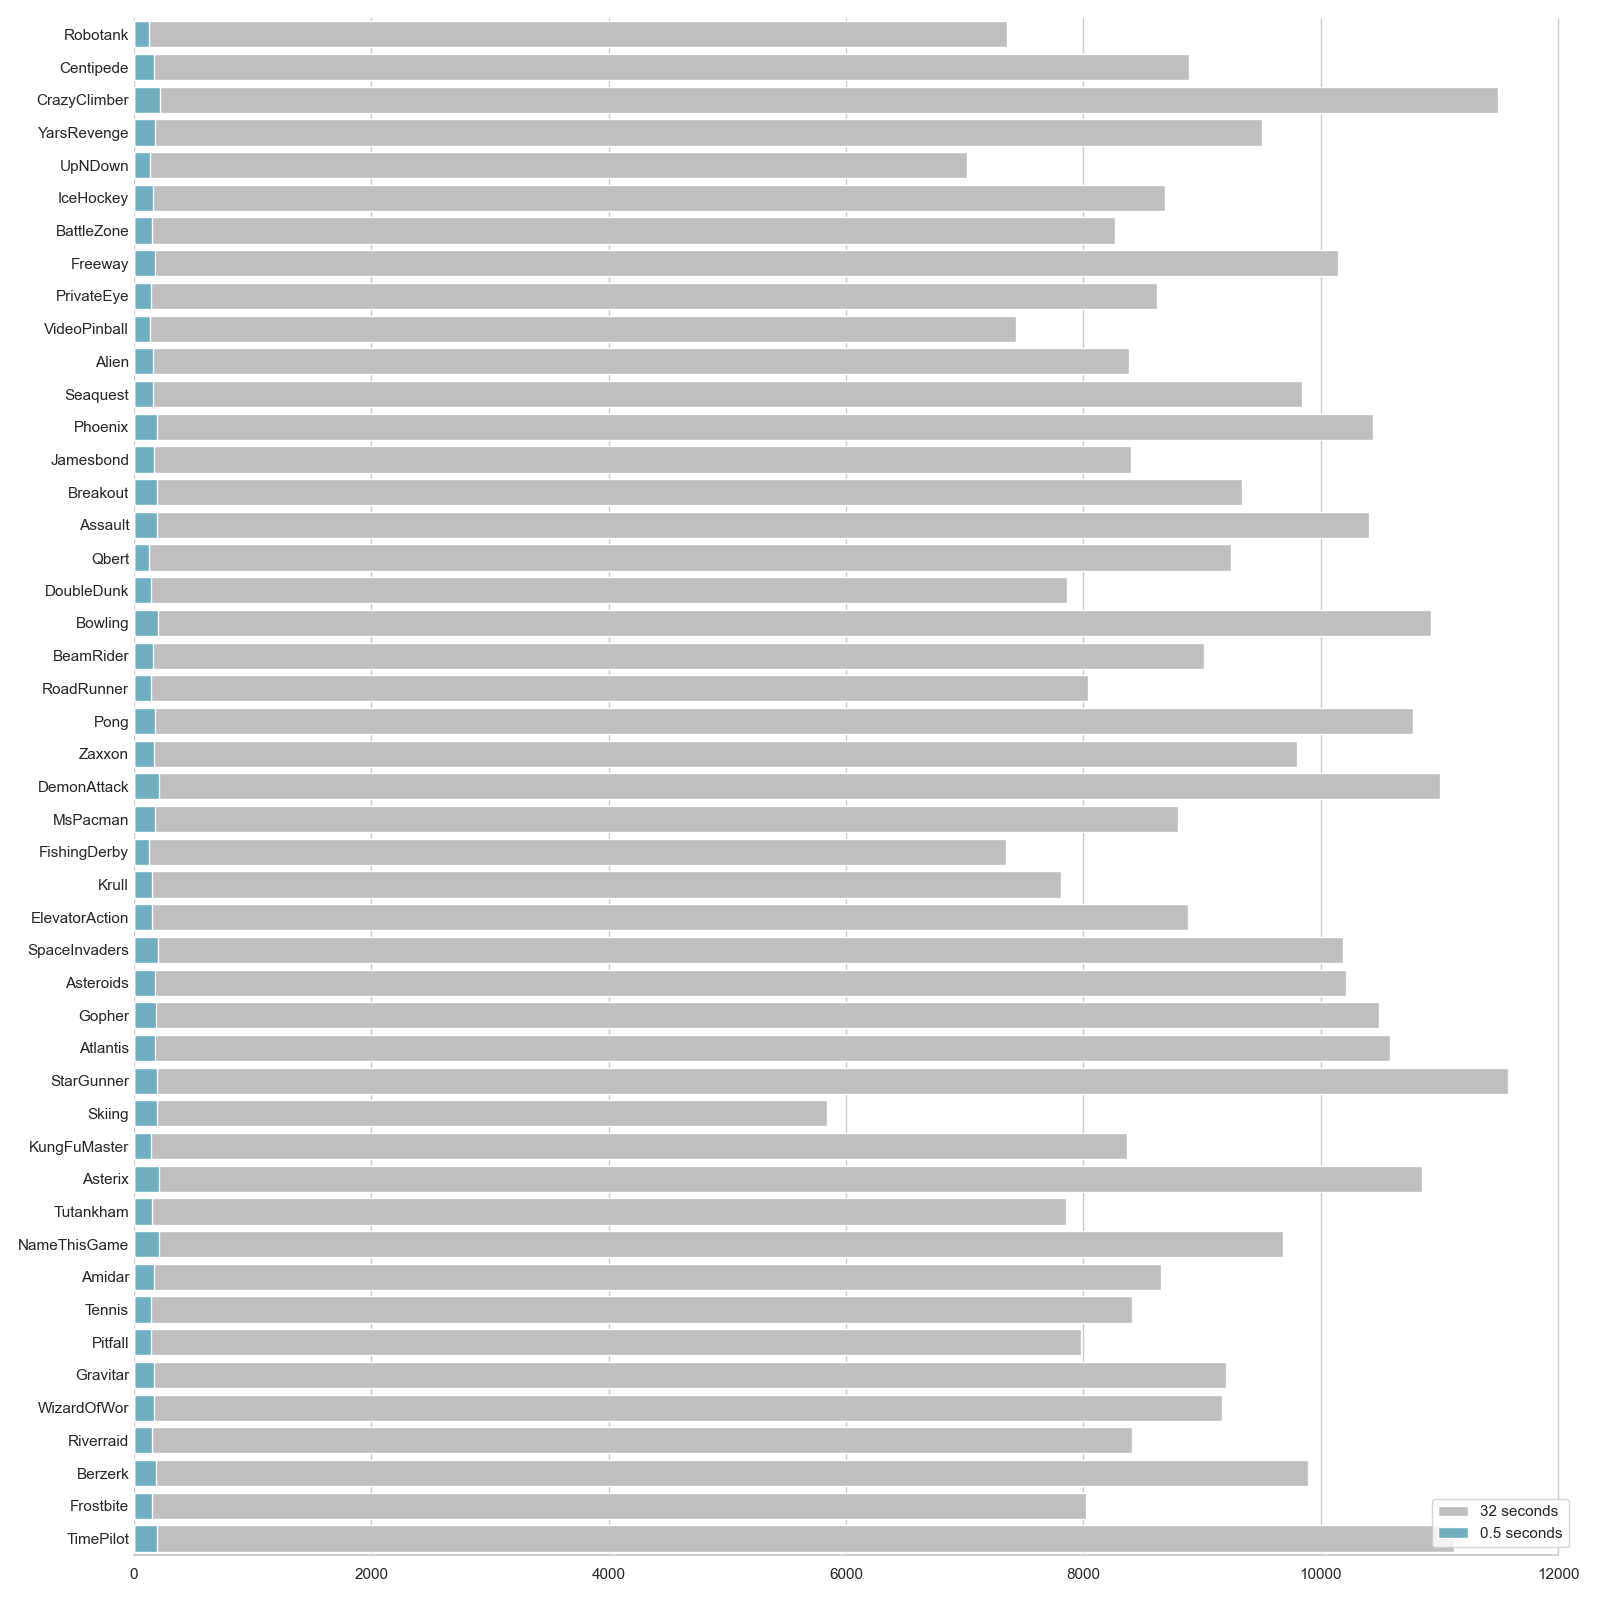
\includegraphics[width=\textwidth]{Pictures/means_nodes_for_32_and_0_5.png}
    \caption{Mean number of expanded nodes during one planning phase for each domain (one run per domain). The comparison is between the 0.5 second RA VAE-IW and 32 second RA VAE-IW.}
    \label{fig:mean_expanded_nodes}
\end{figure*}
\begin{figure*}[ht]
    \centering
    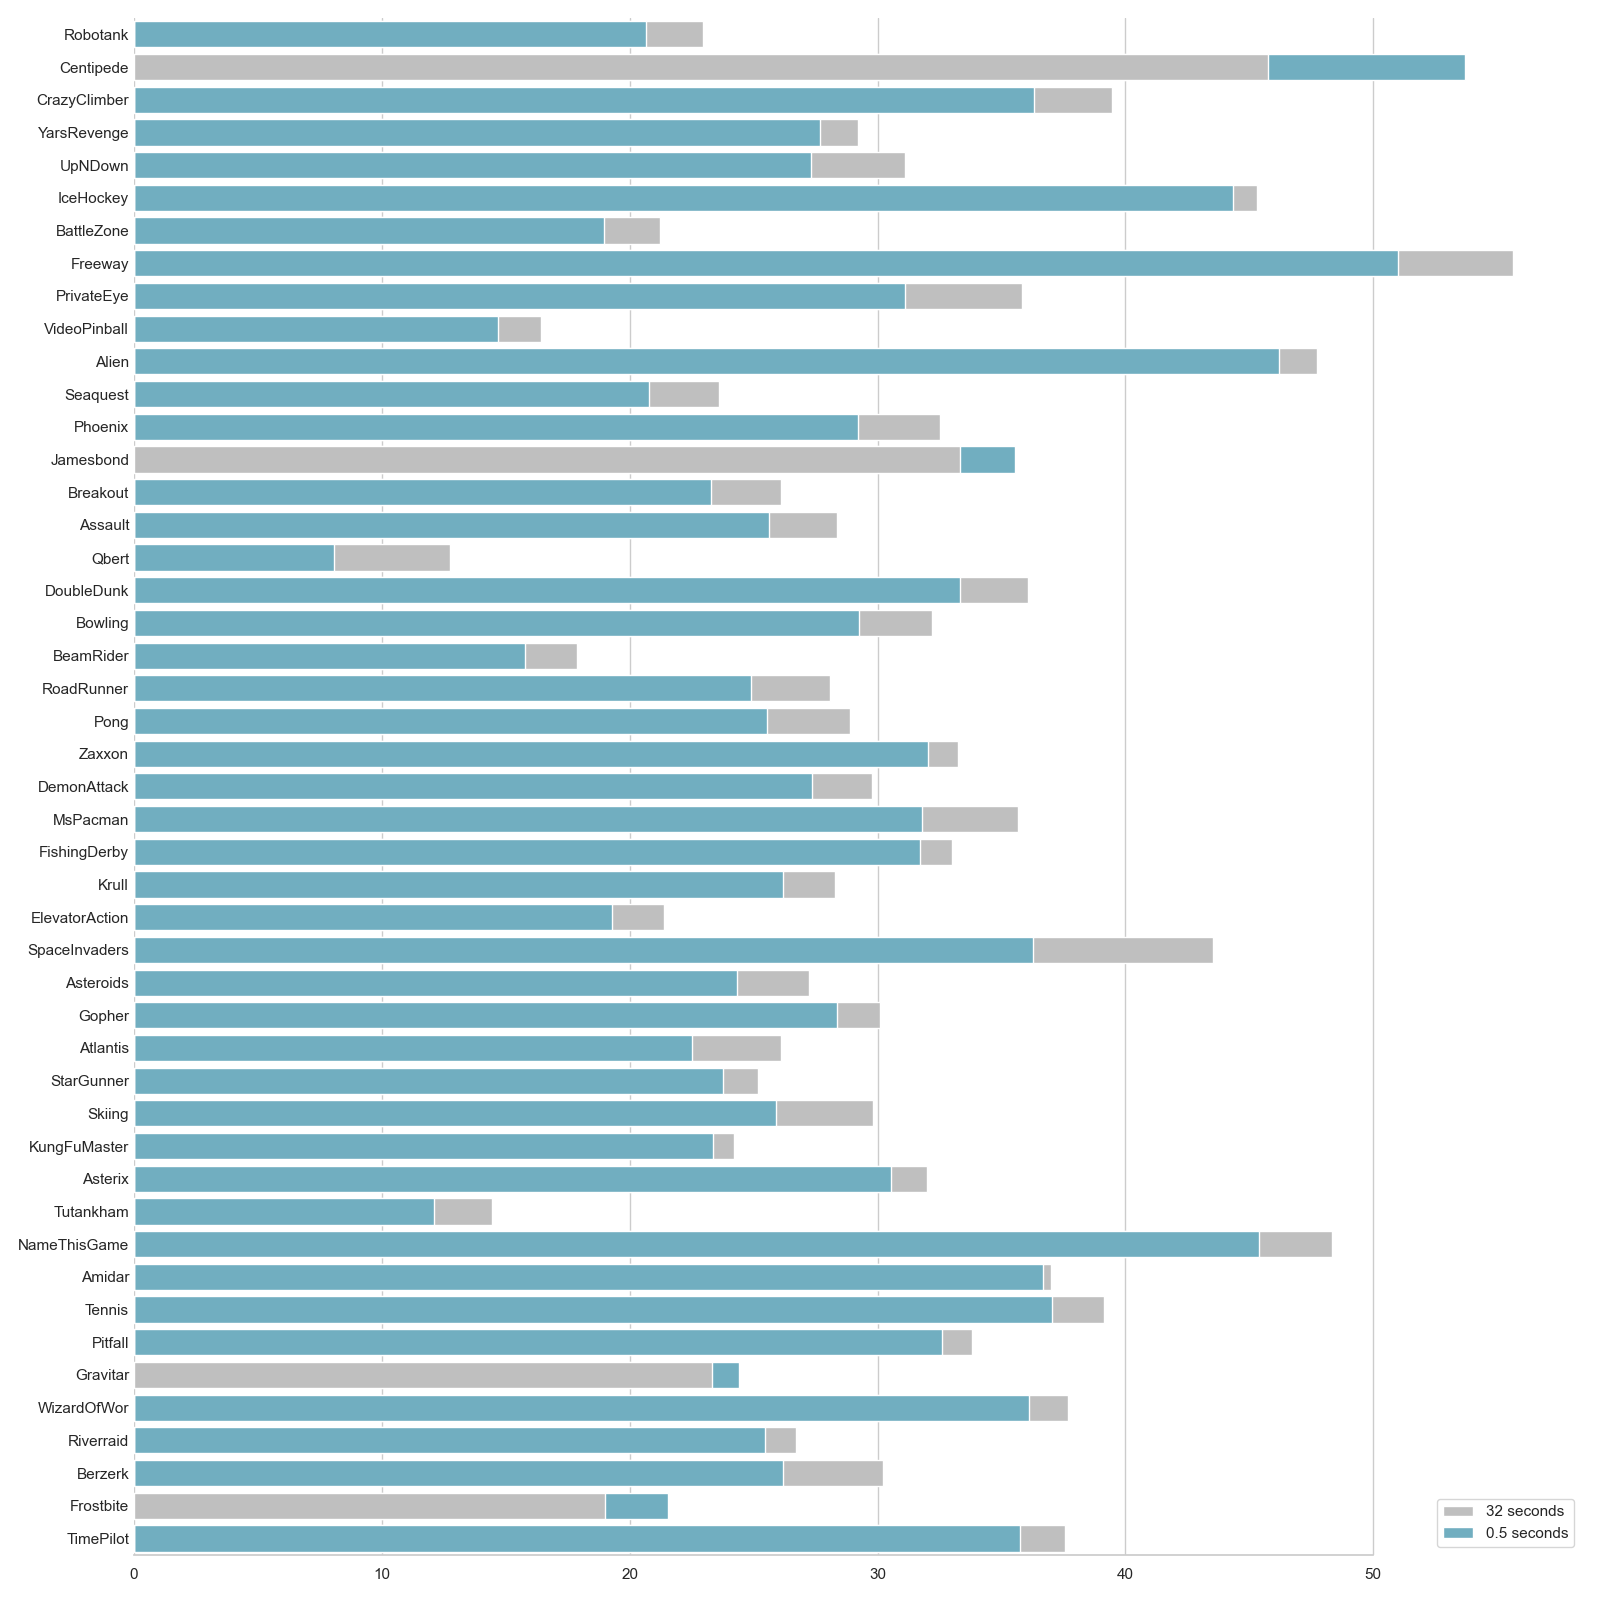
\includegraphics[width=\textwidth]{Pictures/means_depth_for_32_and_0_5.png}
    \caption{Mean of the maximum rollout length for each domain (one run per domain). The comparison is between the 0.5 second RA VAE-IW and 32 second RA VAE-IW.}
    \label{fig:mean_depth_nodes}
\end{figure*}
